\documentclass[10pt,letterpaper]{article}
\usepackage[margin=0.9in]{geometry}
\usepackage{amsmath}
\usepackage{booktabs,multirow}
\usepackage{graphicx}
\usepackage{xcolor}
\usepackage{enumitem}
\usepackage{caption}
\usepackage{microtype}
\usepackage[hidelinks]{hyperref}
\usepackage{orcidlink}
\captionsetup{font=small,labelfont=bf,labelsep=period}
\setlist{itemsep=2pt,topsep=3pt}
\pagestyle{plain}


% Transparency notes: numbered, listed on a Notes page, referenced with \tnote{key}
\newcommand{\tnote}[1]{\textsuperscript{\hyperref[note:#1]{\ref*{note:#1}}}}

\begin{document}

\begin{center}
{\Large\bfseries Evidence-Weighted Confidence: Making an LLM's Confidence Mean Something}\\[6pt]
Issam Zeinoun~\orcidlink{0009-0007-4874-880X} $\cdot$ Independent Researcher $\cdot$ October 2026 $\cdot$ Version 3\\[2pt]{\color{gray}\textsc{Short version}}
\end{center}

\paragraph{Bottom line.} LLM-stated confidence is not a probability. Across five current models judging whether a clinical note supports a diagnosis code, charts the model called 93--99\% certain were correct only 54--72\% of the time. Replacing the stated number with a small fitted logistic regression over the model's verified answers to rule-derived questions fixed this on every model: when the score said 90\% or more, it was right 93--100\% of the time, and the score ranked cases far better (AUROC 0.90--1.00 against 0.59--0.77). The pattern helps in two ways. It makes inexpensive models usable: Claude Haiku 5.5 matched the best frontier result at about 1/15 of the cost. On frontier models it matches the ranking they reach when given the same questions, and adds better calibration, a verified quote behind every answer and a reproducible score; the same prompt that worked on the strongest models failed on GPT-5.4, while the pattern held on all five.

\paragraph{The pattern.} The LLM reads; code decides.
\begin{enumerate}
  \item A rubric of yes / no / \emph{not documented} questions is derived from the rules that govern the decision (here, the ICD-10-CM coding guidelines for E11.22, type 2 diabetes with diabetic CKD): four gates (diabetes type, established CKD, face-to-face visit with a qualified clinician, signed note) and four weighted questions (stage, eGFR history, attribution to diabetes, addressed at this visit).
  \item The LLM answers each question with a verbatim quote; code checks the quote is in the note.
  \item Gates must pass; a logistic regression fitted on about 100 labeled development cases turns the weighted answers into a probability.
\end{enumerate}
Every score therefore comes with an audit trail of quoted evidence, and each weight reads as how much one kind of answer moves the log-odds. The fit is an ordinary logistic regression; no Bayesian inference is used.

\paragraph{Setup.} Pre-registered, with prompts, rubric, weights and thresholds hash-frozen before a single test evaluation per model. 350 synthetic outpatient notes (150 development, 200 held-out test; 117 of the test notes support the code), including copied-forward plans, unclear or conflicting statements, and cases that need rules outside the original rubric. Five models: GPT-5.4, Claude Sonnet 5.5, Claude Haiku 5.5, Gemini 3.8 Flash, Gemini 3.5 Flash-Lite. Three methods per model:
\textbf{A}, the model's stated 0--100 confidence (raw and Platt-recalibrated on development data);
\textbf{C}, the same questions and guidance put in the prompt, with the model told to base its confidence on them;
\textbf{B}, evidence-weighted confidence (the pattern).
C isolates what the fitted scoring adds beyond the questions themselves.

\begin{table}[h]
\centering\footnotesize
\caption{Held-out test (200 cases per model). AUROC / ECE; and, for cases given 90\% or more, number of cases: average confidence $\rightarrow$ share actually correct.}\label{tab:main}
\setlength{\tabcolsep}{3.5pt}
\begin{tabular}{@{}lccc|ccc@{}}
\toprule
 & \multicolumn{3}{c|}{AUROC / ECE} & \multicolumn{3}{c}{Cases given 90\%+: said $\rightarrow$ actual} \\
Model & A (recal.) & C & \textbf{B} & A (raw) & C & \textbf{B} \\
\midrule
GPT-5.4 & 0.59 / 0.05 & 0.48 / 0.37 & \textbf{0.93 / 0.04} & 149: 95\%$\rightarrow$54\% & 191: 97\%$\rightarrow$60\% & 46: \textbf{93\%$\rightarrow$93\%} \\
Claude Sonnet 5.5 & 0.72 / 0.07 & 0.99 / 0.09 & \textbf{0.99 / 0.02} & 39: 93\%$\rightarrow$67\% & 61: 94\%$\rightarrow$100\% & 117: \textbf{97\%$\rightarrow$98\%} \\
Claude Haiku 5.5 & 0.77 / 0.11 & 0.92 / 0.23 & \textbf{0.99 / 0.01} & 31: 93\%$\rightarrow$61\% & 36: 94\%$\rightarrow$89\% & 118: \textbf{98\%$\rightarrow$98\%} \\
Gemini 3.8 Flash & 0.65 / 0.11 & 1.00 / 0.04 & \textbf{1.00 / 0.00} & 183: 97\%$\rightarrow$63\% & 119: 96\%$\rightarrow$98\% & 117: \textbf{100\%$\rightarrow$100\%} \\
Gemini 3.5 Flash-Lite & 0.69 / 0.08 & 0.78 / 0.25 & \textbf{0.90 / 0.05} & 107: 99\%$\rightarrow$72\% & 66: 100\%$\rightarrow$89\% & 44: \textbf{93\%$\rightarrow$93\%} \\
\bottomrule
\end{tabular}
\end{table}

\filbreak
\paragraph{Findings.}
\begin{enumerate}
  \item \textbf{B's confidence means what it says, on every model.} B was the best-calibrated method on all five models (ECE 0.002--0.050), its 90\%+ cases were correct 93--100\% of the time, and its under-10\% cases were correct 0--6\% of the time. B beat recalibrated stated confidence on AUROC by 0.21--0.35 on every model (paired bootstrap intervals all above zero). Recalibration fixes the average of the stated number but not its ranking; for GPT-5.4 it could only reverse it, because the model's confidence pointed the wrong way (AUROC 0.41, below chance), so the recalibrated score almost never exceeds 90\% and cannot route anything (Figure~\ref{fig:rel}).
  \item \textbf{Giving the model the questions is not enough.} With the rubric in the prompt, Sonnet and Gemini 3.8 Flash ranked as well as B (AUROC 0.99--1.00; the pre-registered ``B beats C'' check failed on these two, as predicted for Gemini). GPT-5.4, Haiku and Flash-Lite did not: GPT-5.4 put 191 of 200 cases above 90\% and was right on 60\%. The questions help the model reason; the fitted scoring layer is what makes the number trustworthy across models. On the two strong models B tied C on ranking but was better calibrated (ECE 0.021 vs 0.090 on Sonnet, 0.002 vs 0.036 on Gemini 3.8 Flash), and only B shows the quoted evidence behind each score.
  \item \textbf{Fix the questions, not the model.} An earlier transfer test on harder notes found that the frozen six-question rubric auto-accepted notes written by a nurse, unsigned, or from an e-consult with no patient seen (mean score 0.94--0.99): no question asked about them, and the evidence trail showed it. Adding two gates derived from risk-adjustment rules, with no model change, made B reject all 26 such held-out cases on all five models; C, given the same two questions, got 25 of 26 wrong on GPT-5.4.
  \item \textbf{Inexpensive models become usable.} Claude Haiku 5.5 with B (AUROC 0.994, ECE 0.014; auto-accepted 60\% of cases at 96.7\% precision) matched or beat Claude Sonnet 5.5 with B, at about \$2.82 against \$43.82 for the full run, and was the only model to pass all four pre-registered checks. Gemini 3.5 Flash-Lite with B (AUROC 0.897) outranked every model's own confidence, but was not accurate enough to reach the 95\%-precision auto-accept target; that shortfall was visible on development data before deployment.
\end{enumerate}

\begin{figure}[h]
\centering
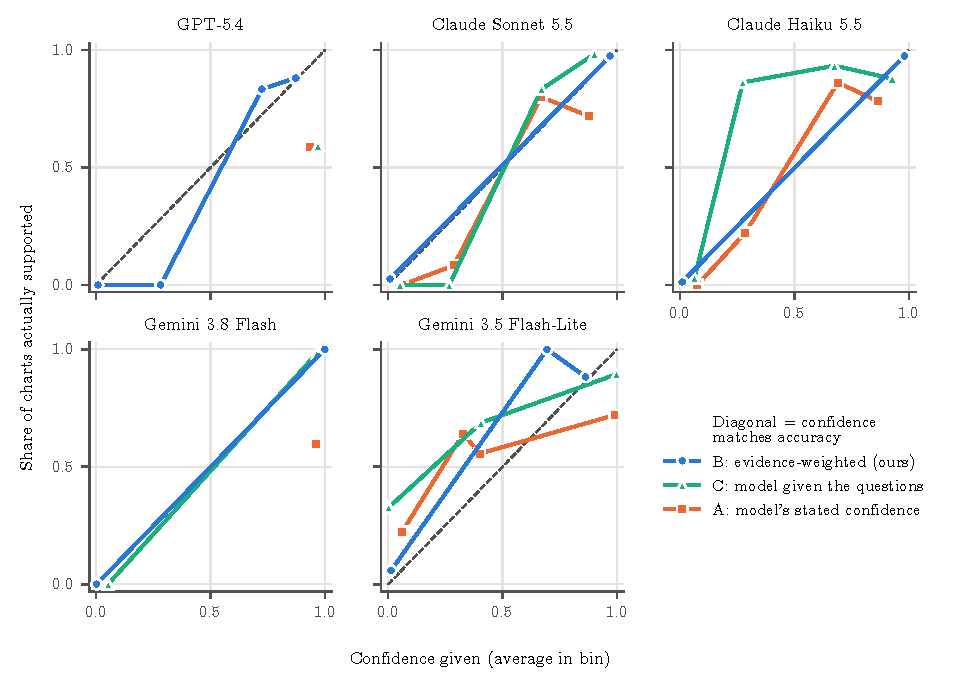
\includegraphics[width=0.86\textwidth]{figures/reliability.pdf}
\caption{Reliability on held-out cases: average confidence given (x) against share actually correct (y), five bins. The diagonal is perfect calibration.}\label{fig:rel}
\end{figure}

\paragraph{Pre-registered checks.} B beat recalibrated A by at least 0.10 AUROC: 5 of 5 models. B calibrated at least as well as A and C: 5 of 5. B beat C on AUROC: 3 of 5 (ties on Sonnet and Gemini 3.8 Flash). B's development threshold held 95\% precision on test: 3 of 5 (GPT-5.4 93.5\%; Flash-Lite had no threshold).

\paragraph{Caveats.} The notes are synthetic, and their labels follow largely from the facts the rubric asks about, which favors B by construction (C gets the same questions to keep the comparison fair). Labels were set by the author with AI assistance.\tnote{coder} One code, 200 test cases, 58\% positive. The notes were generated with Claude, and two Claude models were tested. Three of the five models were added after the pre-registration, each under its own addendum filed before its first call. Models almost never misquoted, so the quote check was barely exercised; the remaining errors are real quotes misread (``see nephrology note'' taken as the condition being addressed). The value of separating silence from contradiction is not measured here.\tnote{contra} Fitted weights reflect correlated answers and should not be read one by one as evidence strengths.

\paragraph{Next.} Real notes labeled by certified coders, more codes with shared family-level rubrics, charts that oversample contradictions, and a semantic check that each quote supports its answer. The full paper gives the method, why the scoring is additive in log-odds, all tables and the algorithm specification; its earlier version, with the method and protocol published before any experiment, and all later versions are at \href{https://doi.org/10.5281/zenodo.23651100}{doi:10.5281/zenodo.23651100}. Code, data, pre-registrations and freeze records: \url{https://github.com/izeinoun/rubric_for_medical_coding}.

\paragraph{Notes.} These notes are given for transparency only. None of them affects the conclusions of this paper.
\begin{enumerate}[label=\arabic*.,ref=\arabic*]
\item\label{note:coder} \textbf{No certified coder.} The label rules were set by the study lead with AI assistance, and one reviewer checked 74 charts using Gemini 3.1 Pro as a reading aid (a Gemini model was also among those tested); no certified coder reviewed the labels. Because every method is scored against the same labels, this does not affect the comparison between methods or the conclusions. Whether the rules match certified coders' practice, for example on copied-forward plan lines, is a question for a study on real charts.
\item\label{note:contra} \textbf{Few documented contradictions.} The charts were balanced by label (supported or not) and by scenario family, not by answer type. A documented other cause for CKD (Q3 ``no'') appears in 5 of 350 charts (2 development, 3 test); contradictions of the gate questions and of Q2 appear in 15--30 charts each. The benefit of keeping silence and contradiction apart is therefore not measured by these studies, and the fitted weight for Q3 ``no'' is set mostly by regularization. This does not affect the conclusions, which are measured on the final supported-or-not decision across all test charts. A follow-up could oversample contradictions for every question.
\end{enumerate}

\end{document}
